%
% Diese Datei nicht einbinden, sondern die einzelnen Absätze an die richtigen Stellen kopieren.
%     
        
    


\section{Raspberry Pi 3}
Der Raspberry Pi ist ein vollständiger Computer in der Größe einer Kreditkarte. Er wird von der nicht profitorientierten Raspberry Pi Foundation entwickelt und in Großbritannien hergestellt. Er besitzt keinen aufgelöteten Speicher, sondern bootet direkt von einer MicroSD-Karte. Die Raspberry Pi Foundation entwickelt auch das offizielle Betriebssystem Pi OS auf Basis von Linux (Debian).

Die dritte Version des Raspberry Pi (3 Mod. B v1.2) hat 1GB RAM und als CPU vier ARM Cortex-A53-Kerne, welche die ARMv8-A-Mikroarchitektur implementieren. Für dieses Modell gibt es aktuell keine offizielle 64-bit-Version von Pi OS.
Die Schnittstellen umfassen MicroUSB für die Stromversorgung, HDMI für die Bildausgabe, 3,5mm Klinke für Audio, RJ-45 (Ethernet), 4x USB 2.0, 40 GPIO-Pins und zwei Flachband-Header für den offiziellen Touchscreen und die offizielle Kamera. \autocite{RaspberryPi1}

Die vierte Version (4 Mod. B) hat eine schnellere CPU mit vier ARM Cortex-A72-Kernen, 2GB bis 4GB RAM, fest verbautes Wi-fi und Bluetooth, schnellere USB 3.0 Anschlüsse, sowie zwei Micro-HDMI-Buchsen. Die Form ist gleich geblieben. \autocite{RaspberryPi2}

\section{Einrichtung}
Für dieses Projekt wurde ein Raspberry Pi 3 verwendet. Als Betriebssystem wurde aufgrund der Spezialisierung auf diese Hardware Pi OS (Build vom 30.10.2021) gewählt. Aus Platzgründen musste der Raspberry Pi per Fernzugriff gesteuert werden. Hierfür wurde zuerst das vorinstallierte realVNC verwendet, später jedoch auf SSH gewechselt. Grund dafür war, dass mit SSH mehrere Verbindungen gleichzeitig aktiv sein können. Zudem ist die Performance unter Last deutlich besser, weil eine grafische Aufbereitung und die Übertragung der Bilddaten entfallen.

\section{Intel Movidius Myriad X}
Der Myriad X der Intel-Tochterfirma Movidius ist eine Vision Processing Unit (VPU), die auf IoT-Anwendungen spezialisiert ist. Sie unterstützt bis zu 8 Kameras mit einer Auflösung von 4k. Sie kann Aufgaben wie Stereosicht und Bildverarbeitung sehr effizient ausführen und ist dabei nicht auf Datentransfers zu externem Speicher angewiesen.

Zusätzlich ist sie mit einer Neural Compute Engine ausgestattet, die ein schnelles und Energieeffizientes Ausführen von Inferenz auf neuralen Netzen ermöglicht. Movidius gibt eine Performance von 1 TOPS (1 Billion Operationen pro Sekunde) an.

\section{Luxonis OAK-D}
Die Luxonis OAK-D ist eine IoT-Kamera, die einen RGB-Sensor und ein Paar Stereosensoren hat. Der Stereosensor nutzt einen Sony IMX378-Sensor und kann Video in 4k aufnehmen. Das Stereopaar nutzt Omnivision OV9282-Sensoren mit einer Auflösung von 1280x800.
Die Sensoren sind direkt mit der integrierten Myriad X VPU verbunden. Stromversorgung und Datentransfer erfolgen über USB-C, wobei sowohl USB 2.0 als auch USB 3.0 unterstützt werden.

Die Kamera wird über die DepthAI-Platform und deren Python-API gesteuert. Hierbei kann der Entwickler selbst entscheiden, welche Sensoren und Funktionen der VPU er in welchem Ausmaß nutzt.

\section{RC522 RFID-Modul}

Das RC552-Modul von NXP Semiconductors ist ein RFID-Transponder, der das 13.56Mhz ISM-Band nutzt und dadurch keine Probleme mit anderen Funkverbindungen verursacht. Es kann über UART, I²C oder SPI kommunizieren und wird mit 3.3V betrieben, passt also auf die GPIO-Pins des Raspberry Pi. Eine Besonderheit ist der Interrupt-Pin, mit dem ein externes Gerät aufgeweckt werden kann, sobald ein RFID-Tag erkannt wird. Es wird mit zwei RFID-Tags geliefert, die beliebig beschrieben und ausgelesen werden können. 

\section{SSH}

Secure Shell ist ein Netzwerkprotokoll, mit dem verschlüselt auf entfernte Rechner zugegriffen werden kann. Der entfernte Rechner muss dafür direkt erreichbar sein (über ein lokales Netzwerk oder eine Portweiterleitung).
SSH ist ein Client-Server-Protokoll, wobei der entfernte Rechner der Server und der lokale Rechner der Client ist. Neben klassischen textbasierten Shells können mit SSH auch verschlüsselte Dateiübertragungen (per SFTP) und grafische Anwendungen (per X11-Forwarding) realisiert werden.


\section{Evaluation der Pipeline}

Die Kennzeichenerkennungspipeline besteht aus folgenden Schritten:
\begin{itemize}
    \item[Laden der kurz zuvor gespeicherten Datei]
    \item[Preprocessing]
    \begin{itemize}
        \item[Umwandlung zu Graustufen]
        \item[Bilateraler Filter]
        \item[Canny-Algorithmus zu Kantenfindung]
        \item[Douglas-Peucker-Algorithmus zur Erkennung von Rechtecken]
        \item[Cropping]
        \item[OCR mit vorgefertigter Lösung]
    \end{itemize}
\end{itemize}

Im ursprünglichen Plan gab es am Anfang dieser Pipeline ein neuronales Netz, mit dem eine erste Eingrenzung des Kennzeichens erfolgen sollte. Dieser Schritt wurde jedoch aufgrund von technischen Problemen entfernt.

Als OCR-Lösung war EasyOCR geplant, weil es trotz geringem Ressourcenaufwand gute Ergebnisse liefert. Dieser Ansatz scheiterte, weil EasyOCR von Torch abhängt, Torch ein 64bit-Betriebssystem voraussetzt und Pi OS für den Raspberry Pi 2 nur als 32bit-Version verfügbar ist.
Die Alternative ist Tesseract, eine OCR-Engine, die ursprünglich von Hewlett-Packard entwickelt wurde. Seit 2005 ist es Open-Source und von 2006 bis 2018 wurde es von Google weiterentwickelt. https://tesseract-ocr.github.io/docs/tesseracticdar2007.pdf

\subsection{Cropping}
Bei 85 von 118 Bildern wurde eine Region als Kennzeichen identifiziert und freigestellt.
Diese ist nicht immer korrekt, es wurden neben Kennzeichen auch Fenster, Ziegelsteine und Straßenschilder freigestellt.
Das ist ein Problem, das durch die Vorschaltung von yolov3 verhindert werden könnte. 



\subsection{OCR}
Beide OCR-Lösungen liefern ungenaue Ergebnisse. Die Plaketten zwischen den Blöcken der Kennzeichen werden oft als Zeichen interpretiert. Genauso wird zwischen den Blöcken manchmal ein Leerzeichen erkannt und manchmal nicht.
Bei einem genauen Vergleich dieser Ergebnisse mit einer Liste von erlaubten Kennzeichen würde daher sehr selten ein Treffer auftreten.

Aus diesem Grund wird stattdessen das Python-Paket \lstinline{thefuzz} verwendet, welches sich die Levenshtein-Distanz zu Nutze macht, um die Ähnlichkeit mehrerer Strings zu quanitfizieren.
Um die Levenshtein-Distanz zwischen zwei Strings zu bestimmen, wird ein String zum Anderen umgeformt. Erlaubte Operationen sind dabei das Einfügen eines neuen Zeichens und das Entfernen eines bestehenden Zeichens.
Die minimal benötigte Anzahl dieser Operationen ist die Levenshtein-Distanz.

Hieraus wird ein prozentualer Wert abgeleitet, der die Genauigkeit der Erkennung wiederspiegelt.
Für die finale Evaluation mit dieser Methode wurde ein Threshold von 45\% gewählt, um das gelesene Kennzeichen als richtig einzuordnen.

Mit easyOCR wurden 28 von 85 Kennzeichen richtig gelesen, mit Tesseract 17.
\begin{figure}[h]
	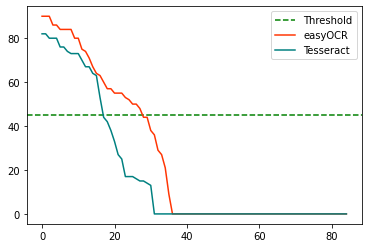
\includegraphics[width=8cm]{./img/evaluation_fuzzy_ratio.svg}
	\caption{Evaluation mit fuzzy_ratio}
\end{figure}

Neben dem vollständigen Fuzzy Matching können mit der Funktion \lstinline{fuzz.partial_ratio()} auch Substrings berücksichtigt werden.
Das ist sinnvoll, um beispielsweise die Namen von Autohäusern aus den OCR-Ergebnissen herauszufiltern.
Mit dieser Methode (Threshold 45\%) liest easyOCR 31 von 85 Kennzeichen richtig, Tesseract 22.
\begin{figure}[h]
	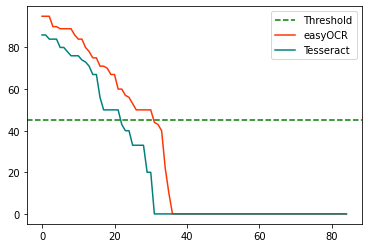
\includegraphics[width=8cm]{./img/evaluation_partial_ratio.svg}
	\caption{Evaluation mit partial_ratio}
\end{figure}


Abgesehen von den bestehenden Methoden zum Vergleich mehrerer Strings wurde auch ein spezialisierter Ansatz entwickelt. Sowohl easyOCR als auch Tesseract haben die Schwäche, dass sie manchmal die Blöcke der Kennzeichen vertauschen. Um dieses Problem zu umgehen, wurde folgende, auf das vorliegende Problem spezialisierte, Funktion zur Evaluation entwickelt:
% Keine Ahnung wie ich das schreiben soll, das da halt:
% 
\begin{lstlisting} 
def custom_match(read, label):	
    for x in label:
        if x not in read:
            return 0
    return 100
\end{lstlisting}     
% Bild dazu: eval_custom
Die Werte 0 und 100 dienen der einheitlichen Visualisierung. \lstinline{read} ist der Text, den die OCR-Lösung erkannt hat. \lstinline{label} ist das Label des jeweiligen Bildes in der Form \lstinline{OG AE 1337}. Die leerzeichengetrennten Teile des Labels werden durch Python in jeweils einzelnen Schleifendurchläufen behandelt.
\begin{figure}[h]
	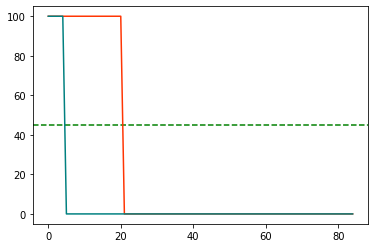
\includegraphics[width=8cm]{./img/evaluation_custom_matcher.svg}
	\caption{Evaluation mit eigener Funktion}
\end{figure}


Es ist zu beachten, dass nicht alle im Vorigen Schritt freigestellten Bildsegmente auch wirklich Kennzeichen sind. Ein Mensch könnte an dieser Stelle also auch keine perfekte Leistung erreichen. 

\subsection{Laufzeit}

Für eine praktische Anwendung darf die Laufzeit der gesamten Pipeline nicht zu lang sein.
%Wenn die Laufzeit der Pipeline, also die Verzögerung zwischen der Aufnahme zweier Bilder \delta t ist,
%dann wird das 

Erstens sollte die Zeit zwischen dem Auftauchen des Autos vor der Kamera und dem ersten Scan konsistent sein,
zweitens kann die Pipeline im gleichen Zeitraum mehrmals ausgeführt werden und so trotz ungenauen Modellen gute Ergebnisse erzielen.
Die Laufzeit hängt direkt von der verwendeten Hardware ab.

Zur Evaluation wird die Dauer der einzelnen Schritte (Cropping und OCR) gemessen und zu Durchschnitten aggregiert.

Auf dem selbst erstellten Datensatz wurde mit einem Lenovo Thinkpad T580 (Intel i7-8850U) für das Cropping durchschnittlich 1,37 Sekunden,
für die Texterkennung mit easyOCR 2,27 Sekunden und für die Bilderkennung mit Tesseract 2,67 Sekunden benötigt.
Das entspricht einer Gesamtlaufzeit von rund 4 Sekunden, also etwa 15 Bildern pro Minute.

Wird jedoch stattdessen ein Raspberry Pi 3 verwendet, steigt die Laufzeit auf durchschnittlich 14,87 Sekunden für das Cropping und 17,62 Sekunden für die Texterkennung mit Tesseract.
EasyOCR wurde nicht evaluiert, weil es nicht mit der verwendeten Version von Pi OS kompatibel ist.






\section{Darknet und YOLO v3 (Technologie)}
	
	Darknet ist ein in C und CUDA geschriebenes Framework für neuronale Netze, das auf die Verarbeitung von Bilddaten spezialisiert ist. Es wird von Joseph Chet Redmon entwickelt. \autocite{darknet13}
	
	Zusammen mit dem Darknet-Framework werden auch vorkonfigurierte und -trainierte Modelle bereitgestellt. Eines davon ist YOLO (You only look once). Es klassifiziert und lokalisiert Objekte in Bildern mit sehr hoher Performance. In der dritten Version wird ein mAP von 57.9 erreicht. Ein Modell besteht aus einer Konfigurationsdatei und Gewichten. \autocite{yolov3}
	
	Inferenz mit Darknet-Modellen kann auch direkt auf der Myriad X VPU ausgeführt werden, wenn sie in ein proprietäres Format konvertiert werden.
	
	
\section{YOLO v3 (Umsetzung)}

Um in den aufgenommenen Bildern die Kennzeichen einzugrenzen, sollte zuerst YOLO v3 zum Einsatz kommen. Aufgrund der geringen Menge an selbst verfügbaren Daten und der hohen Ähnlichkeit zu anderen Aufgaben, wurde hier ein Transfer-Learning-Ansatz angewandt. Grundlage war die yolov3-Konfiguration von Redmon und die auf dem COCO-Datensatz erstellten Gewichte.

Um das Transfer-Learning auszuführen, muss zuerst Darknet kompiliert werden. Das Training kann zwar auf einer CPU ausgeführt werden, das hätte jedoch in diesem Fall zu Laufzeiten von mehreren Tagen geführt. Eine GPU ist also für das Training unabdingbar.
Hierbei gab es aufgrund der proprietären Nvidia-Grafiktreiber und den zusätzlichen Paketen CUDA und CUDNN große Schwierigkeiten.
Nachdem diese überwunden waren, konnte ein Modell in etwa zwei Stunden trainiert werden. Inferenz auf einem einzelnen Bild dauert im CPU-Modus auf einem i7 8850U mehr als 20 Sekunden. Für Inferenz mit dem Raspberry Pi muss also unbedingt die Myriad X VPU verwendet werden, die in der OAK-D Kamera verbaut ist. Luxonis erreicht mit dieser Hardware und tiny YOLO v4 stabile 30fps. \autocite{Luxonis1}.
Um auf der OAK-D ausgeführt zu werden, muss das Darknet-Modell zuerst in das .pb-Format von Tensorflow umgewandelt werden.
Von dort aus muss es in das Format "Intermediate Representation" von OpenVino konvertiert werden und über eine proprietäre API zu einem Blobfile.
Dieser Schritt war trotz großem Aufwand nicht erfolgreich. Die API hat unerklärte Fehler geworfen. Nach mehreren Tagen Aufwand wurde die Entscheidung getroffen, den ersten Schritt der geplanten Pipeline zu entfernen und die geometrische Lösung zum ersten Schritt zu machen.

